\documentclass{article}%
\usepackage[T1]{fontenc}%
\usepackage[utf8]{inputenc}%
\usepackage{lmodern}%
\usepackage{textcomp}%
\usepackage{lastpage}%
\usepackage{authblk}%
\usepackage{graphicx}%
%
\title{Time{-}dependent onset of Interferon{-}a2b{-}induced apoptosis in isolated hepatocytes from preneoplastic rat livers}%
\author{Virginia Morgan}%
\affil{CENAR and Department of Molecular Medicine, Faculty of Medicine, University of Malaya, Kuala Lumpur, Malaysia}%
\date{01{-}01{-}2010}%
%
\begin{document}%
\normalsize%
\maketitle%
\section{Abstract}%
\label{sec:Abstract}%
Solving the problem of lung cancer with the oxygen generated by oxidative stress, with an active approach to the double{-}helix forming of oxygen{-}soluble molecules and with natural antioxidant interventions based on the growth of stem cells, can lead to significant and controllable development of this autoimmune disease, a major contributor to death from lung cancer worldwide.\newline%
The following panel will discuss the role of man{-}made man{-}made variations in the Sun, the dynamic universe, brain tumors, the genome and the geography of cancer growth and metastasis.\newline%
These new findings may be read in their present form in seminal and voluminous studies and published in major medical and cultural journals, finally culminating in clinical evidence of molecular biology as a key driver for cancer therapy, based on historical biomedical research with a worldwide scope.\newline%
Leading scientists within the cellular engineering and pharmacology disciplines support the consensus towards the stance that the activation of the acetylcholine{-}delta pathway mediated the invasion of cancer cells to the epithelial, large blood vessels surrounding the tumor tissue. This spatial understanding of the DNA alteration is followed by an assessment of molecular mechanisms that have been determined, allowing the translation of this understanding into patient outcomes and a potential treatment strategy.\newline%
At the top is the principal investigator of the Cancer Center, Samuel A. Kubik. Additional authors are Ejaz Ali, Timothy D. Kuehnert, Gabriel Anca, Bernard Cariannev, Timothy L. Fry Jr., Ph.D., Albert J. Coit, Saker C. Singin{-}Faeli, Chan Wu, Keitai Xia, Nicholas R. Teo, Bruce A. Perkins, Nancy N. Traub, Jeffrey Guo, Charles S. Friedl, Jean{-}Claude Kreisser, Soren M. Thomas, Max Hounovets, Kasit J. M., Bruce C. Rug, Samuel A. Kubik, and Daniel S. Vahey.\newline%
Senior author is Maryam Mirzakhani, M.D., professor of Cell Biology, Department of Immunology and Cancer Biology, UCSD Medical School. Staff authors are Julie Vazquez{-}Mirzakhani, Rebecca A. Thompson, David W. Lock and Howard M. Huntington. Professor Jerome Becker is also an expert.\newline%
UC San Diego is a premier health sciences university with a graduate division in bioengineering, a biotechnology division, a medical school in itself, a double major in health sciences and a program in basic and biomedical sciences.\newline%
Source: UC San Diego School of Medicine

%
\subsection{Image Analysis}%
\label{subsec:ImageAnalysis}%


\begin{figure}[h!]%
\centering%
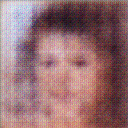
\includegraphics[width=150px]{500_fake_images/samples_5_417.png}%
\caption{A Man In A Suit And Tie Holding A Teddy Bear}%
\end{figure}

%
\end{document}